

\section{METHODOLOGY}
\subsection{Software Development Life Cycle}
\justify

The Verification and Validation (VNV) approach in software development, often referred to as the V-Model, adopts a structured and parallel methodology where each phase of development has a corresponding testing phase, forming a V-shaped structure. Beginning with requirements analysis and system design, the model progresses through coding, unit testing, integration testing, system testing, and finally acceptance testing. Unlike the iterative cycles of Agile, the VNV model follows a sequential path, emphasizing the importance of systematic testing at each stage to ensure the software's compliance with specified requirements. This model is preferred for projects with well-defined requirements, providing a systematic framework for development and testing activities, ultimately ensuring a robust and thoroughly validated software product. \\
\vspace{0.2 in}
\begin{figure}[h]
    \centering
    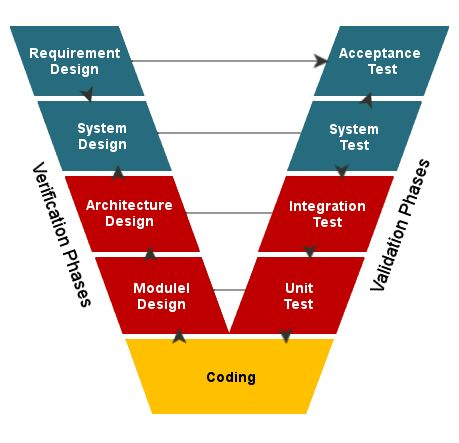
\includegraphics[width= 3in ]{img/VnV.jpg}
    \caption{\textit{VNV Model}}
\end{figure}
